\documentclass[conference]{IEEEtran}
\usepackage{amsmath,amssymb}
\usepackage{graphicx}
\usepackage{booktabs}
\usepackage{siunitx}
\usepackage{hyperref}
\usepackage{cite}
\usepackage{bm}

\graphicspath{{plots/}}

\title{ADCS Homework 2}
\author{John Zhang}

\begin{document}
\maketitle

% ------------------------------------------------------------------
\section{Safe Mode}
\label{sec:safe_mode}

\subsection{Inertia Perturbation}

The ISS nominal principal moments of inertia are
$I_{xx} = \SI{1.280e8}{\kilo\gram\meter\squared}$,
$I_{yy} = \SI{1.070e8}{\kilo\gram\meter\squared}$,
$I_{zz} = \SI{2.010e8}{\kilo\gram\meter\squared}$~\cite{nasa_iss}.
To ensure the solar panel normal ($+Z$ body) is not aligned with a principal
axis, the inertia is perturbed via eigendecomposition:
\begin{equation}
  J = V D V^T, \quad
  \tilde{D} = D(I + \text{diag}(d)), \quad
  \tilde{V} = V \exp(\hat{v}),
\end{equation}
where $d \sim \mathcal{N}(0, 0.03^2 I)$ perturbs eigenvalues by a few percent
and $v \sim \mathcal{N}(0, (3^\circ)^2 I)$ tilts the principal axes by a few
degrees.  The perturbed inertia is $\tilde{J} = \tilde{V}\tilde{D}\tilde{V}^T$.

The resulting perturbed principal moments are:
$I_1 = \SI{1.086e8}{}$, $I_2 = \SI{1.275e8}{}$, $I_3 = \SI{2.049e8}{\kilo\gram\meter\squared}$.
The angular momentum vector $J\bm{\omega}$ is misaligned from $\bm{\omega}$ by
$1.75^\circ$, confirming $+Z$ is not a principal axis.

\subsection{Desired Angular Velocity}

The desired spin is \SI{10}{RPM} about the solar panel normal ($+Z$ body):
\begin{equation}
  \bm{\omega}_d = \frac{10 \times 2\pi}{60} \hat{z}
  = [0, 0, 1.0472]^T~\si{\radian/\second}.
\end{equation}

\subsection{Rotor Momentum via Superspin and Dynamic Balance}

The rotor angular momentum $\bm{h}$ is computed to satisfy two conditions:
\begin{enumerate}
  \item \textbf{Dynamic balance:}
    $\bm{\omega} \times (J\bm{\omega} + \bm{h}) = 0$,
    so the gyrostat equilibrium is torque-free.
  \item \textbf{Superspin:}
    The effective spin-axis inertia $\lambda$ satisfies
    $\lambda / I_{\perp,\max} \geq 1.2$,
    ensuring passive stability against transverse perturbations.
\end{enumerate}

The effective spin-axis inertia is:
\begin{equation}
  \lambda = \frac{(\bm{h} + J\bm{\omega}) \cdot \hat{\omega}}{|\bm{\omega}|}
  = \SI{2.044e8}{\kilo\gram\meter\squared}.
\end{equation}
The maximum transverse inertia is $I_{\perp,\max} = \SI{1.280e8}{\kilo\gram\meter\squared}$,
giving an inertia ratio of $\lambda / I_{\perp,\max} = 1.60 \geq 1.2$.

The computed rotor momentum is
$\bm{h} = [+6.43 \times 10^6,\; +1.26 \times 10^6,\; 0]^T~\si{\kilo\gram\meter\squared/\second}$
with $|\bm{h}| = \SI{6.55e6}{\kilo\gram\meter\squared/\second}$.
The dynamic balance residual $|\bm{\omega} \times (J\bm{\omega} + \bm{h})| < 10^{-10}$
confirms the equilibrium condition.

\subsection{Gyrostat Simulation}

The torque-free gyrostat equation is:
\begin{equation}
  J\dot{\bm{\omega}} + \bm{\omega} \times (J\bm{\omega} + \bm{h}) = 0.
\end{equation}
Coupled with quaternion kinematics, this is integrated using DOP853 (8th-order
Dormand--Prince) with $\text{rtol} = 10^{-12}$.

The estimated nutation period is
\begin{equation}
  T_{\text{nut}} = \frac{2\pi}{\omega_s} \frac{\lambda}{|\lambda - I_\perp|}
  \approx \SI{14.2}{\second}.
\end{equation}

Four cases are simulated for $10 T_{\text{nut}} \approx \SI{142}{\second}$:
\begin{itemize}
  \item \textbf{Case A:} Exact equilibrium initial conditions
  \item \textbf{Case B:} 1\% transverse angular velocity perturbation
  \item \textbf{Case C:} 5\% transverse perturbation
  \item \textbf{Case D:} No rotor ($\bm{h}=0$), 1\% perturbation
\end{itemize}

\begin{figure}[t]
  \centering
  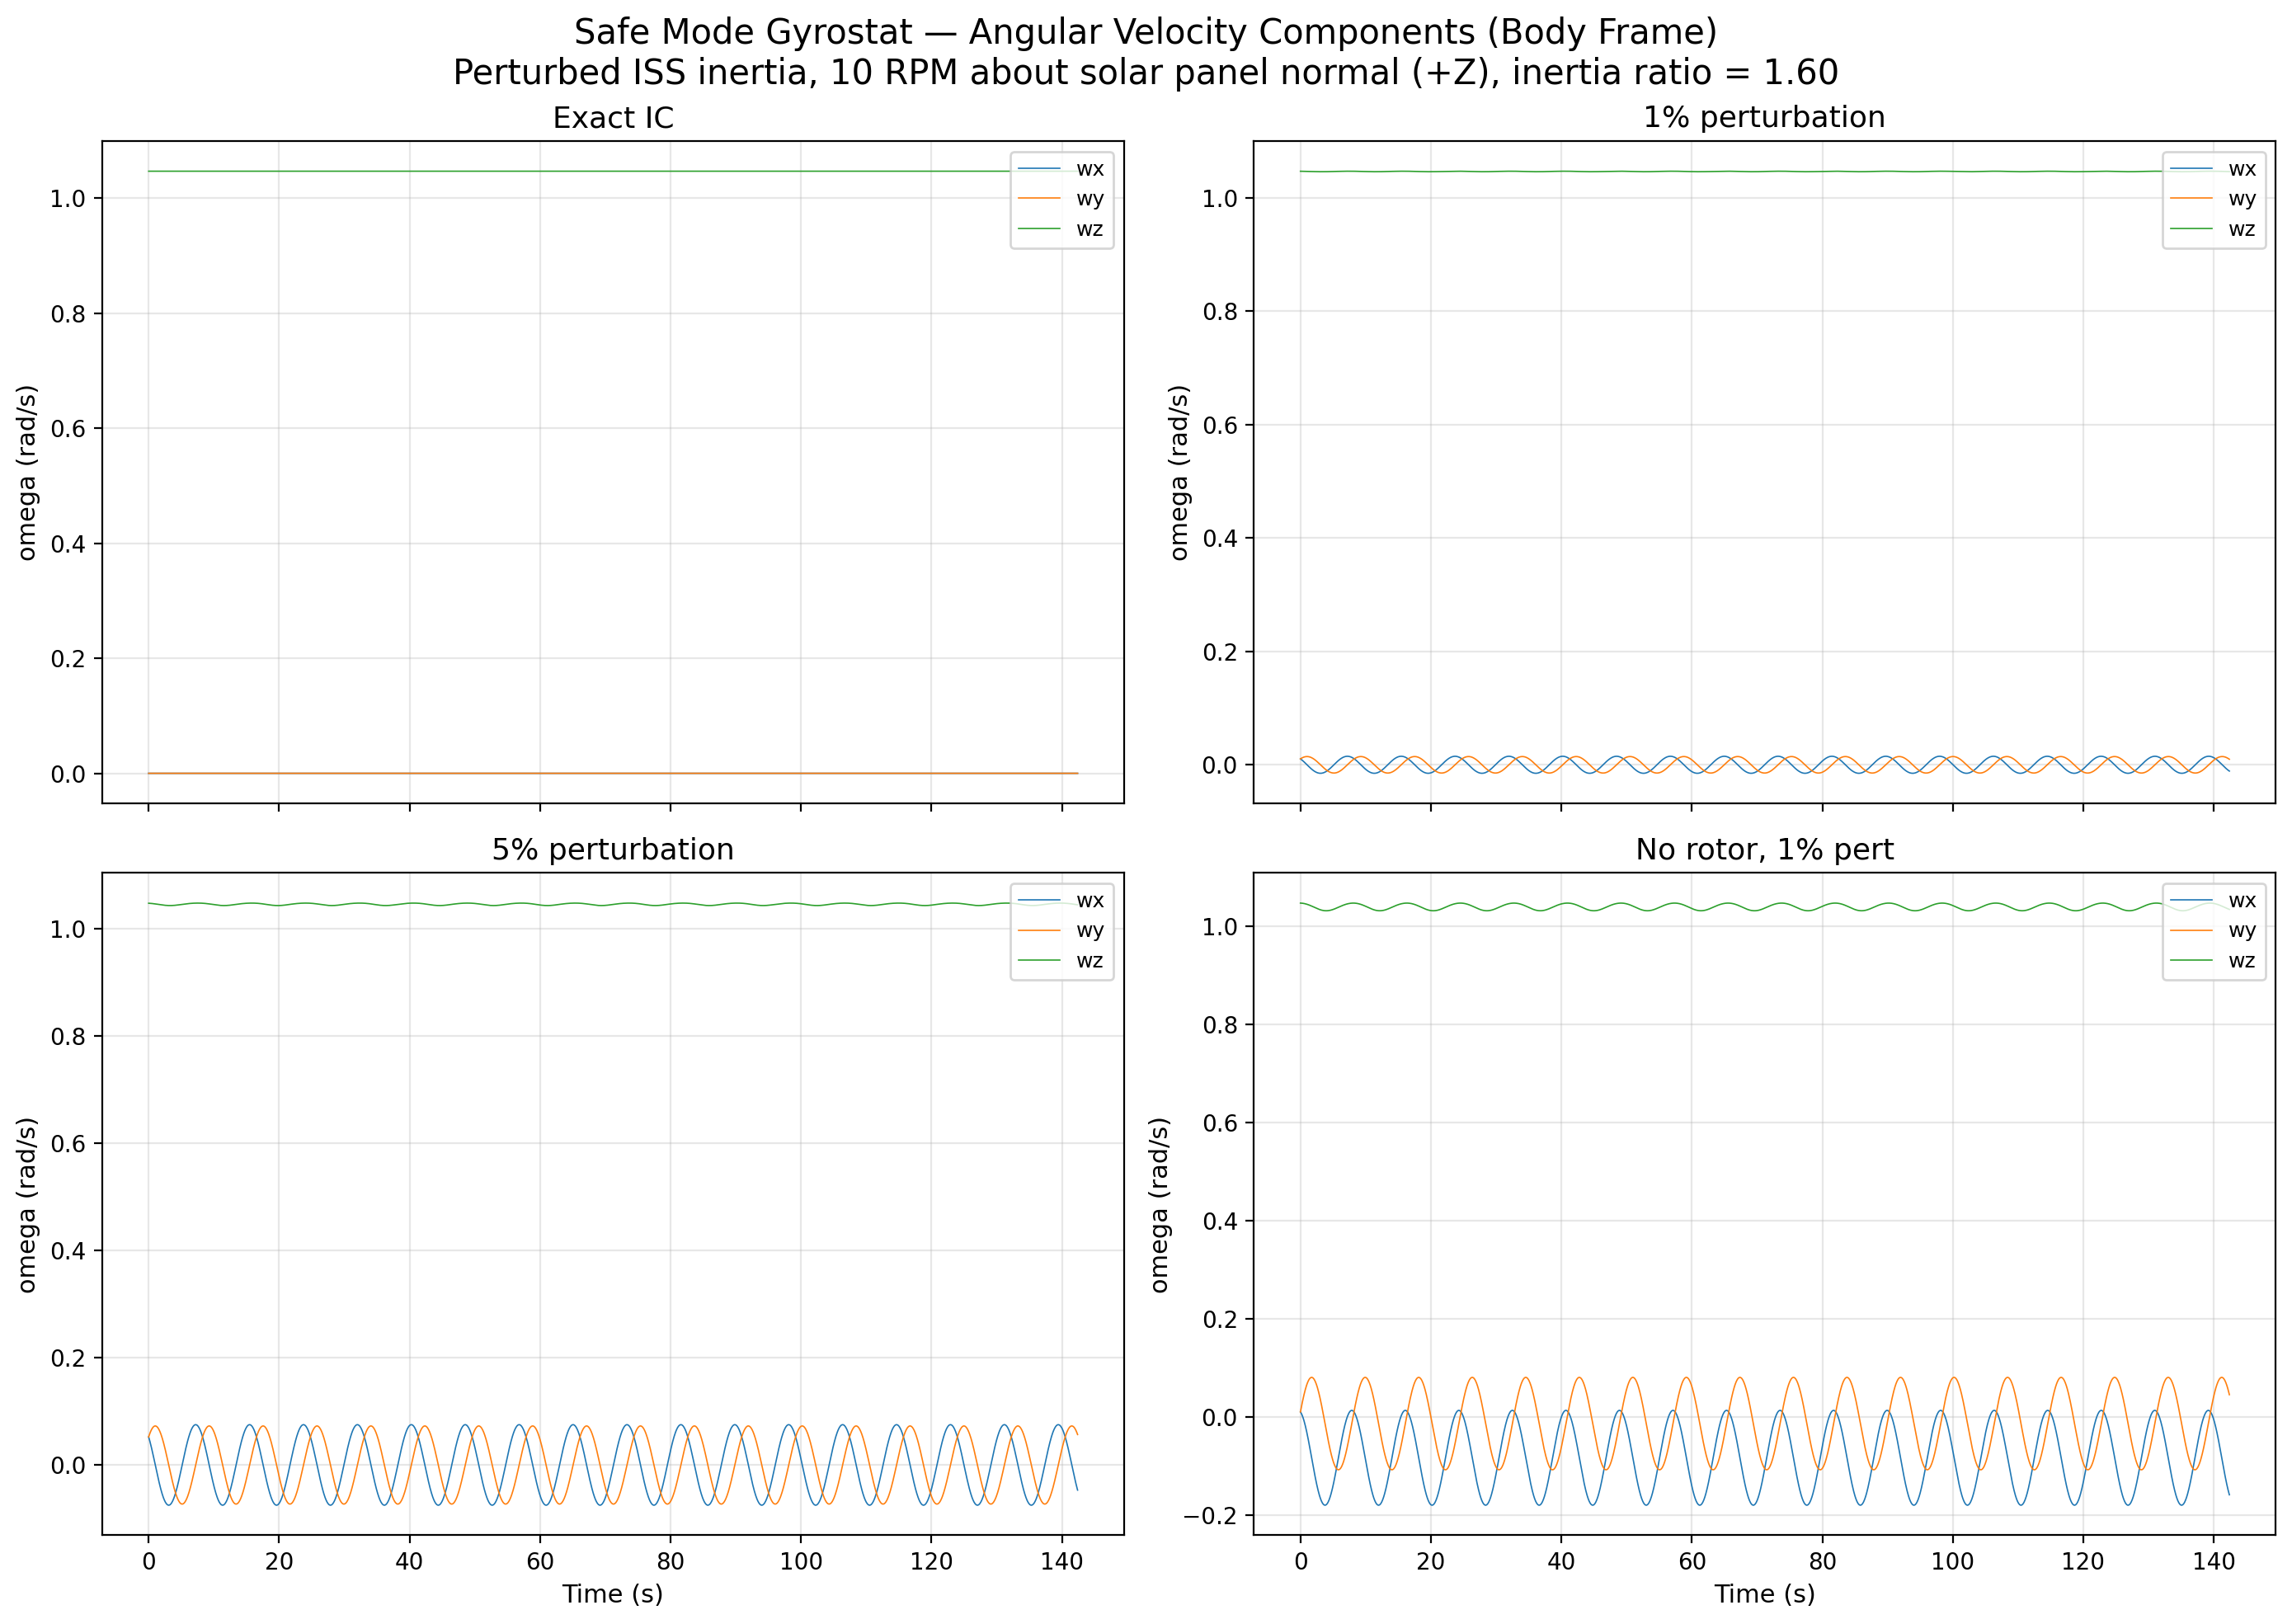
\includegraphics[width=\columnwidth]{safe_mode_omega.png}
  \caption{Angular velocity components for four simulation cases.  With the
    gyrostat rotor (Cases A--C), transverse rates remain bounded; without
    the rotor (Case D), the intermediate-axis instability causes divergence.}
  \label{fig:safe_omega}
\end{figure}

\begin{figure}[t]
  \centering
  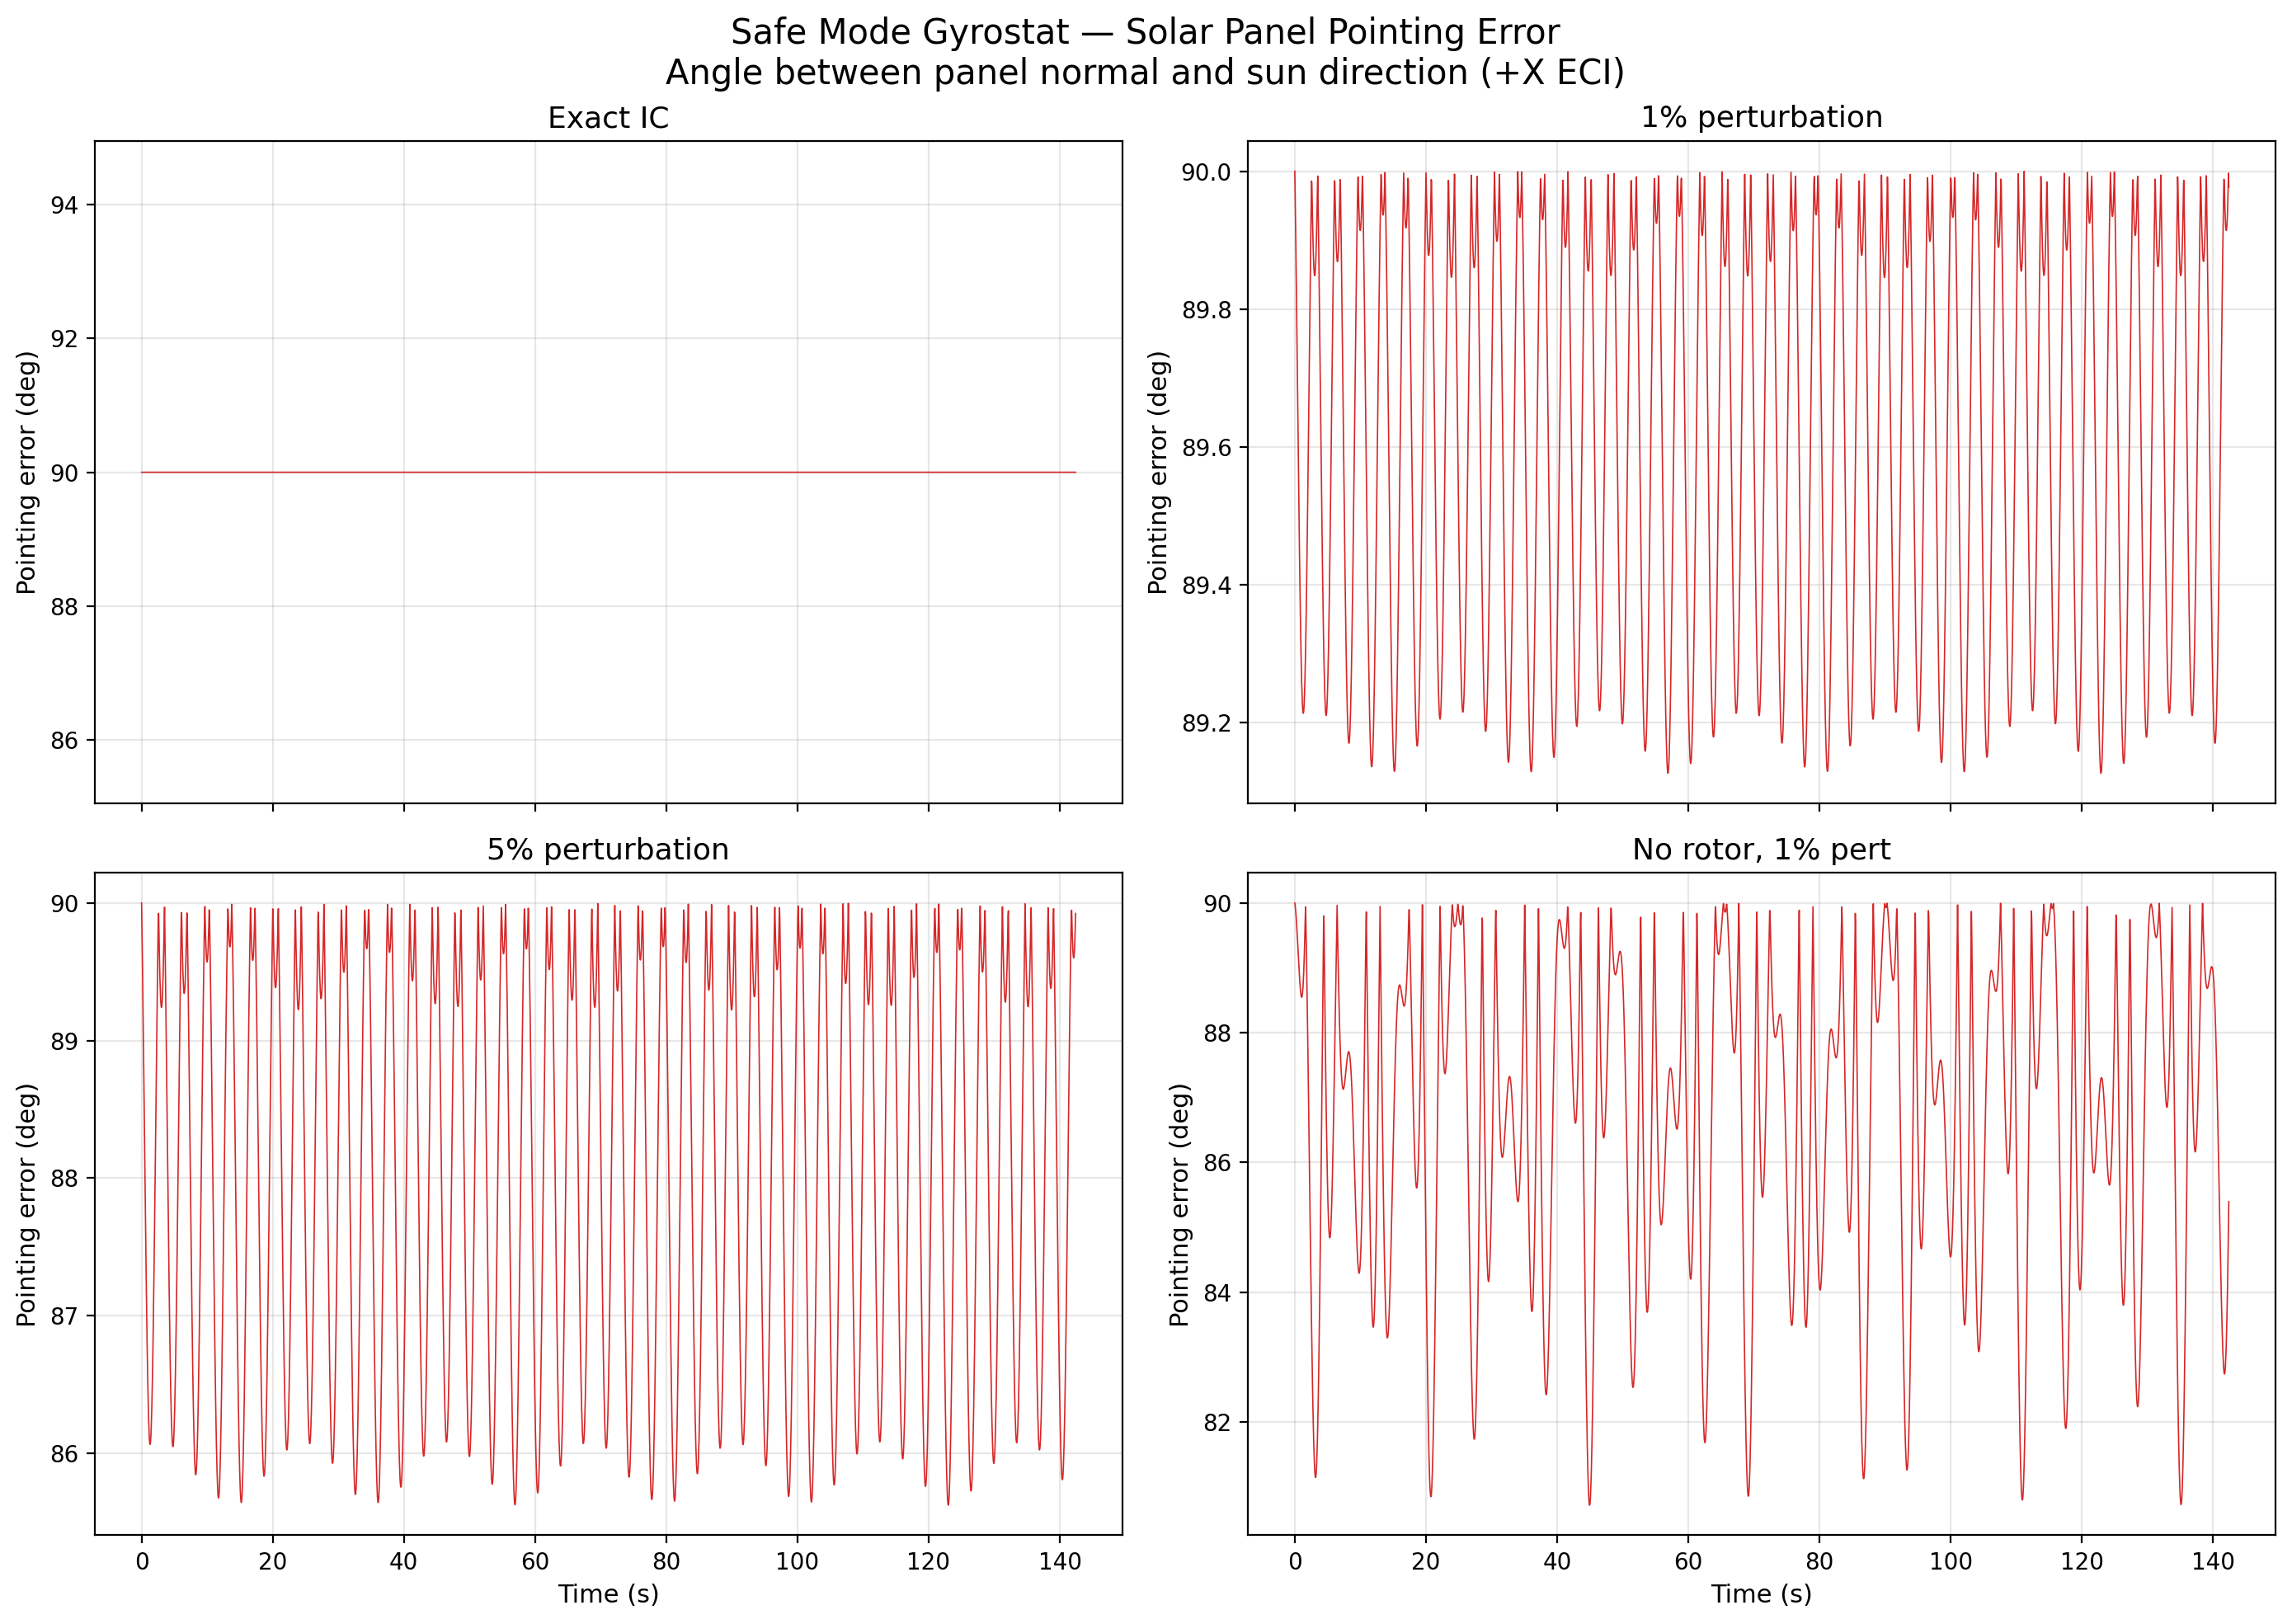
\includegraphics[width=\columnwidth]{safe_mode_pointing.png}
  \caption{Solar panel pointing error (angle between body $+Z$ and sun
    direction).  The gyrostat maintains sub-degree pointing for Cases A--B
    and bounded error for Case C, while Case D (no rotor) diverges.}
  \label{fig:safe_pointing}
\end{figure}

Fig.~\ref{fig:safe_omega} shows the angular velocity histories.
Cases A--C demonstrate bounded nutation with the gyrostat rotor, while
Case D (no rotor) shows the well-known intermediate-axis instability.
Fig.~\ref{fig:safe_pointing} shows the corresponding pointing errors:
the gyrostat maintains stable sun-pointing with bounded nutation even
under 5\% perturbation, whereas the uncontrolled case diverges rapidly.

\begin{figure}[t]
  \centering
  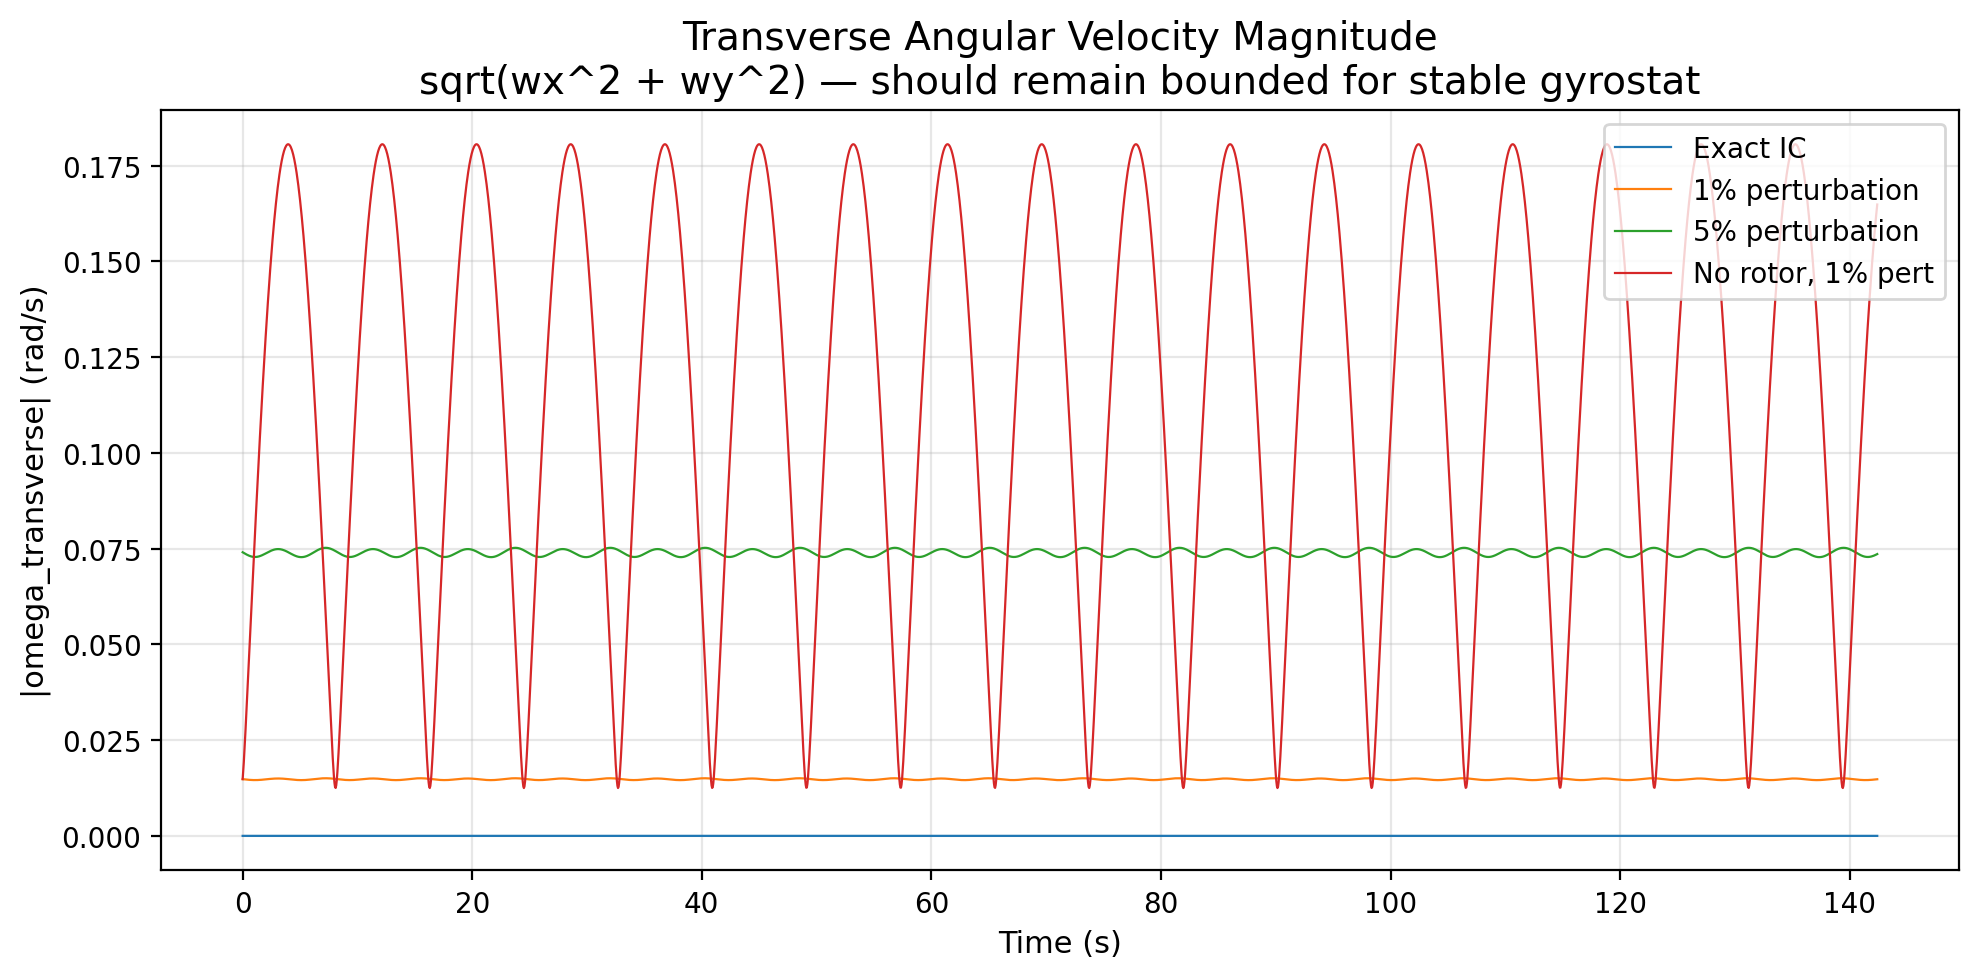
\includegraphics[width=\columnwidth]{safe_mode_transverse.png}
  \caption{Transverse angular velocity magnitude $\sqrt{\omega_x^2 + \omega_y^2}$.
    The gyrostat cases remain bounded (stable nutation) while Case D grows.}
  \label{fig:safe_transverse}
\end{figure}

% ------------------------------------------------------------------
\section{Spacecraft Dynamics}
\label{sec:dynamics}

Gyrostat dynamics are coupled to the orbit simulation from HW1.  The state
vector now includes position $\bm{R}$, velocity $\bm{V}$, attitude quaternion
$\bm{q}$, angular velocity $\bm{\omega}$, and rotor momentum $\bm{h}$.
The simulation uses the \texttt{mujoco\_orbit} framework, which couples
MuJoCo's multibody dynamics with orbital propagation including $J_2$,
atmospheric drag, and solar radiation pressure.

Three reaction wheels (aligned with body $X$, $Y$, $Z$) store the rotor
momentum computed in Section~\ref{sec:safe_mode}.  The same perturbed
inertia and 1\% transverse angular velocity perturbation are used.

The sun vector is assumed parallel to $+X$ in ECI coordinates.  The initial
attitude places the solar panel normal ($+Z$ body) toward the sun.

\begin{figure}[t]
  \centering
  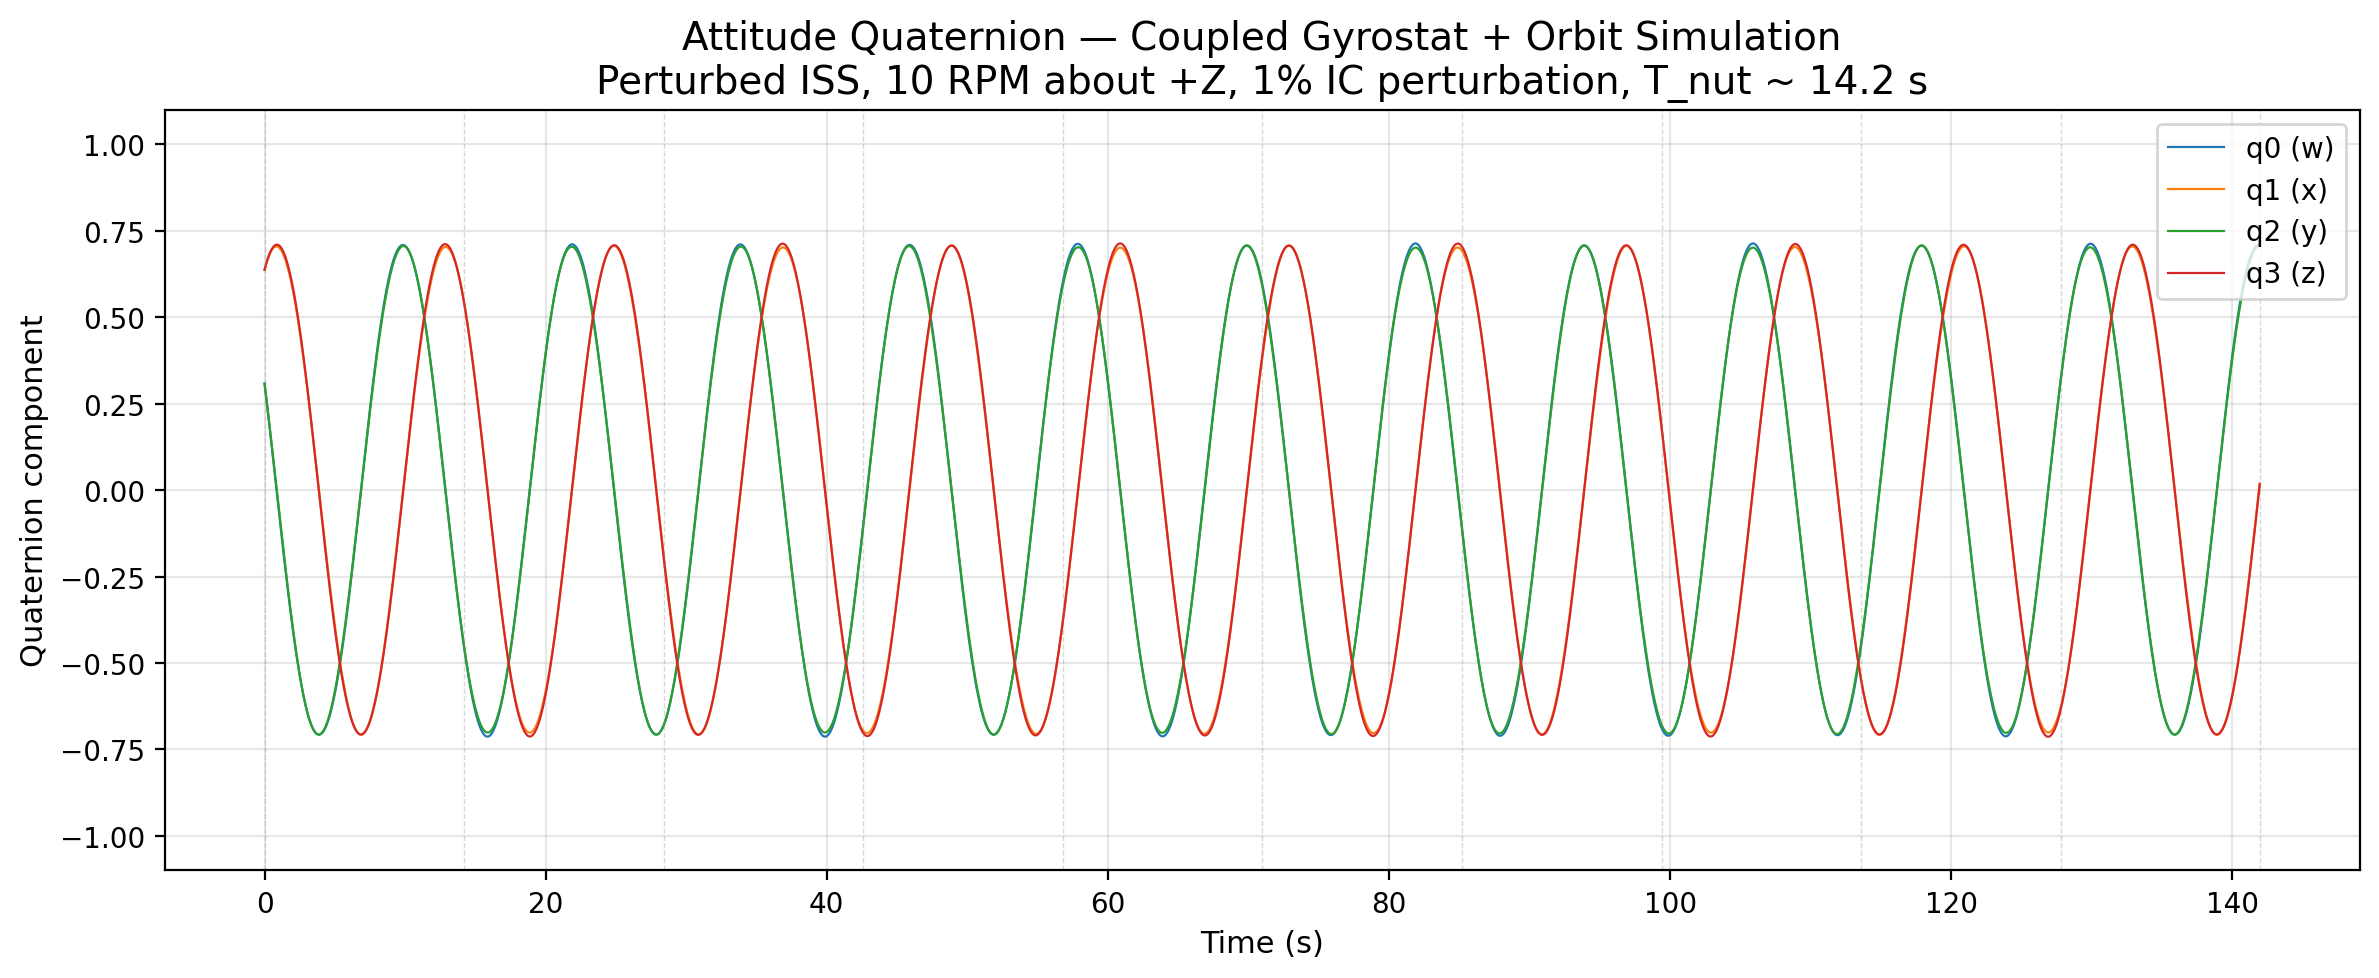
\includegraphics[width=\columnwidth]{spacecraft_dynamics_quaternion.png}
  \caption{Attitude quaternion components during the coupled gyrostat--orbit
    simulation over 10 nutation periods ($T_{\text{nut}} \approx \SI{14.2}{\second}$).}
  \label{fig:dyn_quat}
\end{figure}

\begin{figure}[t]
  \centering
  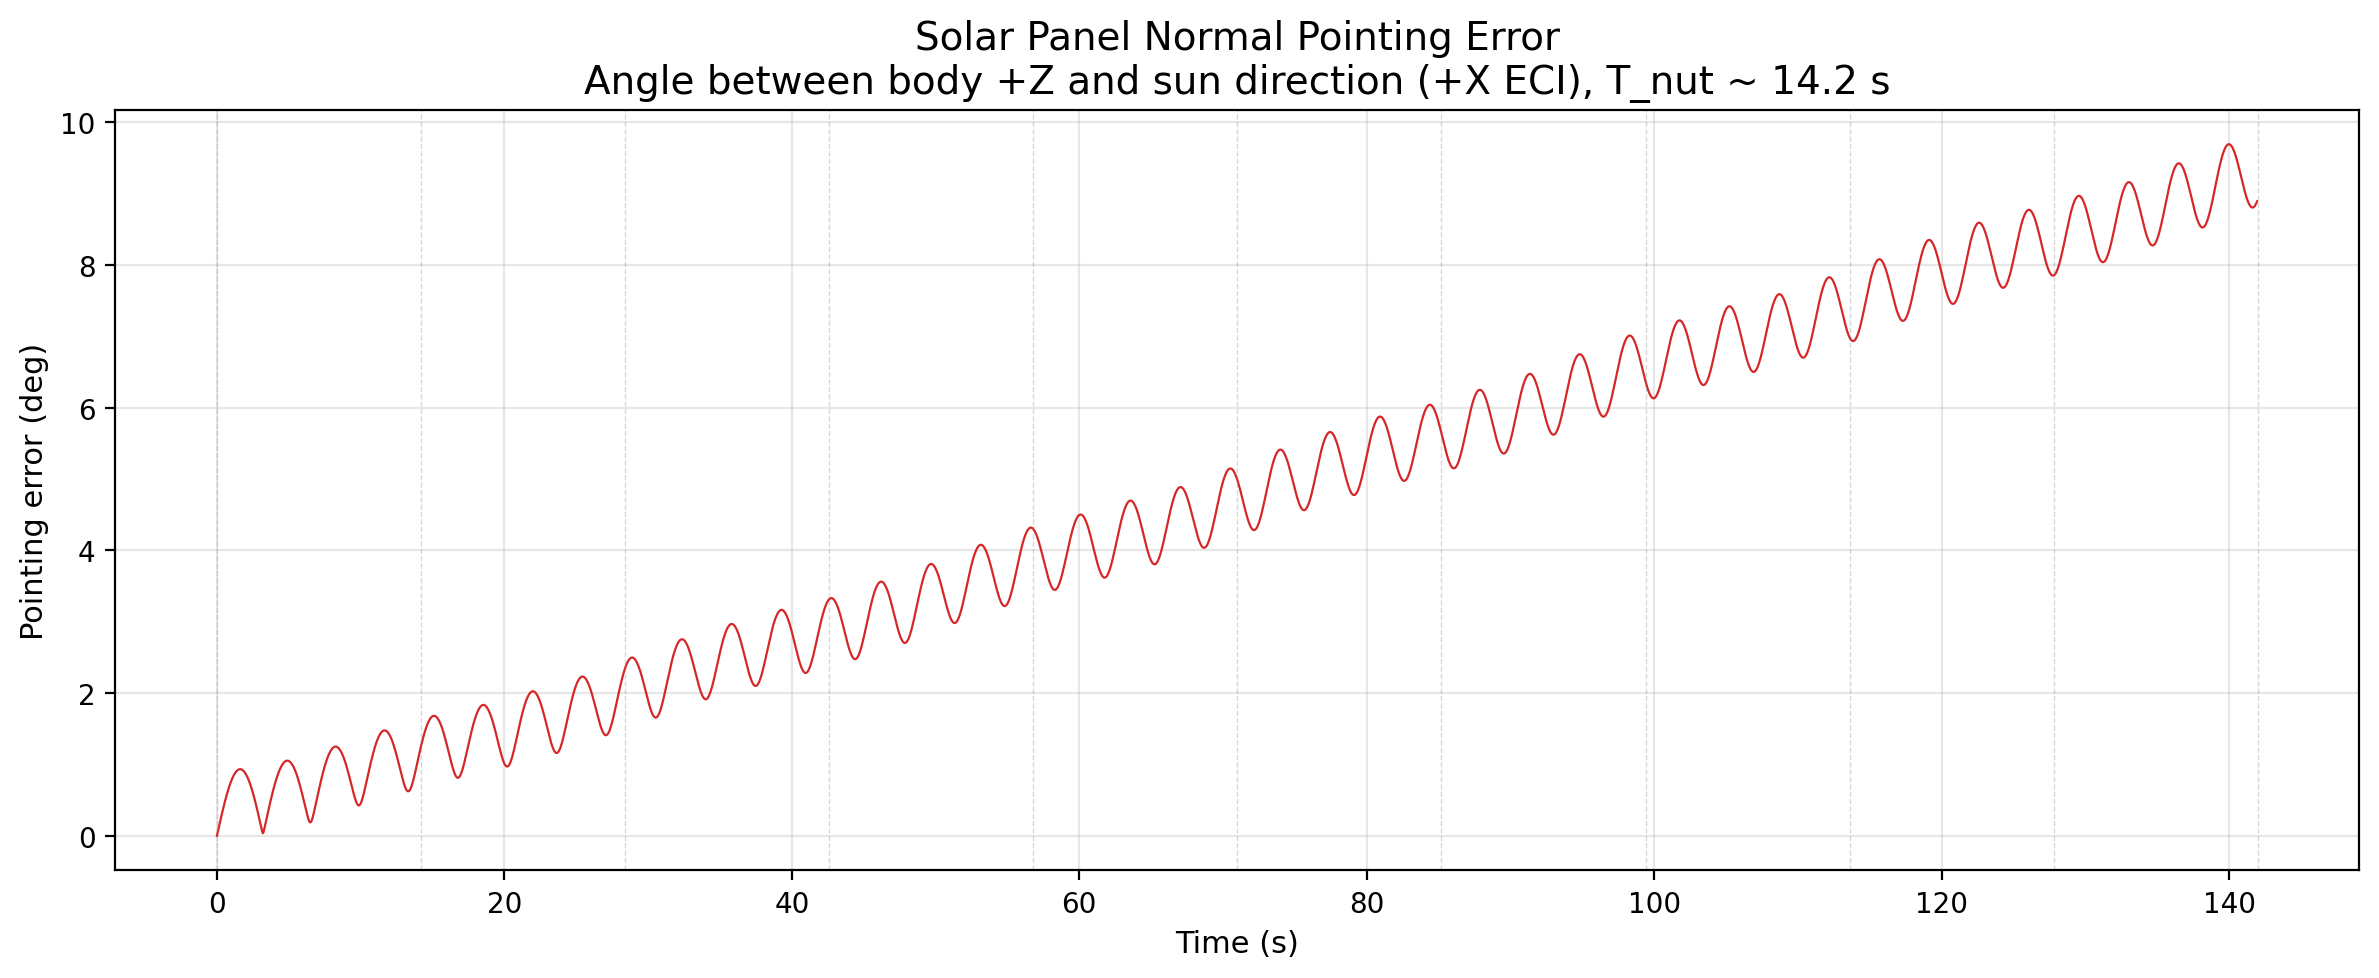
\includegraphics[width=\columnwidth]{spacecraft_dynamics_pointing.png}
  \caption{Solar panel normal pointing error during coupled simulation.
    The error remains bounded below $\sim$$10^\circ$, consistent with the
    nutation amplitude from the 1\% perturbation.}
  \label{fig:dyn_pointing}
\end{figure}

Fig.~\ref{fig:dyn_quat} shows the quaternion evolution, which exhibits
the expected nutation oscillation.  Fig.~\ref{fig:dyn_pointing} shows the
pointing error remains bounded below $\sim$$10^\circ$, consistent with
the safe-mode analysis.  The final pointing error is $8.89^\circ$ with a
maximum of $9.69^\circ$, demonstrating that the gyrostat spin stabilization
maintains approximate sun-pointing even in the presence of orbital coupling
and environmental disturbances.

% ------------------------------------------------------------------
\section{Attitude Sensors}
\label{sec:sensors}

Five attitude sensors are modeled based on ISS flight hardware and
representative specifications from the literature.

\subsection{Sensor Specifications}

\begin{table}[t]
\centering
\caption{Attitude Sensor Specifications}
\label{tab:sensors}
\begin{tabular}{@{}lll@{}}
\toprule
\textbf{Sensor} & \textbf{Parameter} & \textbf{Value} \\
\midrule
Gyroscope & ARW & \SI{0.002}{\degree/\sqrt{hr}} \\
(GG1320AN) & Bias instability & \SI{0.003}{\degree/hr} \\
\midrule
Star Tracker & Cross-boresight & \SI{5}{arcsec} \\
(SED36) & Roll & \SI{25}{arcsec} \\
\midrule
Sun Sensor & Accuracy & \SI{0.05}{\degree} \\
(Adcole) & & \\
\midrule
Magnetometer & Noise density & \SI{30}{nT/\sqrt{Hz}} \\
(HMC2003) & At 10 Hz & \SI{94.9}{nT} \\
\midrule
Horizon Sensor & Accuracy & \SI{0.1}{\degree} \\
(Barnes 13-230) & & \\
\bottomrule
\end{tabular}
\end{table}

\subsection{Covariance Derivations}

\textbf{Rate Gyroscope:}
The angle random walk (ARW) gives the white-noise spectral density:
$\text{ARW} = \SI{0.002}{\degree/\sqrt{hr}} = \SI{5.818e-7}{rad/\sqrt{s}}$.
The per-sample rate noise standard deviation is
$\sigma_\omega = \text{ARW}/\sqrt{\Delta t}$, yielding the covariance
$R_\text{gyro} = (\text{ARW}^2/\Delta t)\, I_3$.
Bias is modeled as a constant offset with
$\sigma_b = \SI{1.454e-8}{rad/s}$.

\textbf{Star Tracker:}
Cross-boresight accuracy of \SI{5}{arcsec} ($\sigma_{xy} = \SI{2.424e-5}{rad}$)
and roll accuracy of \SI{25}{arcsec} ($\sigma_z = \SI{1.212e-4}{rad}$).
The angular error covariance in the sensor frame is
$R_\text{star} = \text{diag}(\sigma_{xy}^2, \sigma_{xy}^2, \sigma_z^2)$,
rotated to the body frame via the sensor mounting matrix.

\textbf{Sun Sensor:}
Isotropic angular noise with $\sigma = 0.05^\circ = \SI{8.727e-4}{rad}$.
The direction-vector covariance for Wahba's problem uses
$\sigma_v^2 = \sigma^2$.

\textbf{Magnetometer:}
At 10 Hz bandwidth, $\sigma_B = 30\sqrt{10} \approx \SI{94.9}{nT}$ per axis.
The direction accuracy depends on field magnitude:
$\sigma_\text{dir} = \sigma_B / |B|$.
At $|B| = \SI{35}{\micro T}$: $\sigma_\text{dir} = 0.155^\circ$.

\textbf{Horizon Sensor:}
Isotropic angular noise with $\sigma = 0.1^\circ = \SI{1.745e-3}{rad}$.

\subsection{Monte Carlo Validation}

A Monte Carlo study with $N = 10{,}000$ samples validates that the simulated
measurement errors match the design covariances.

\begin{figure}[t]
  \centering
  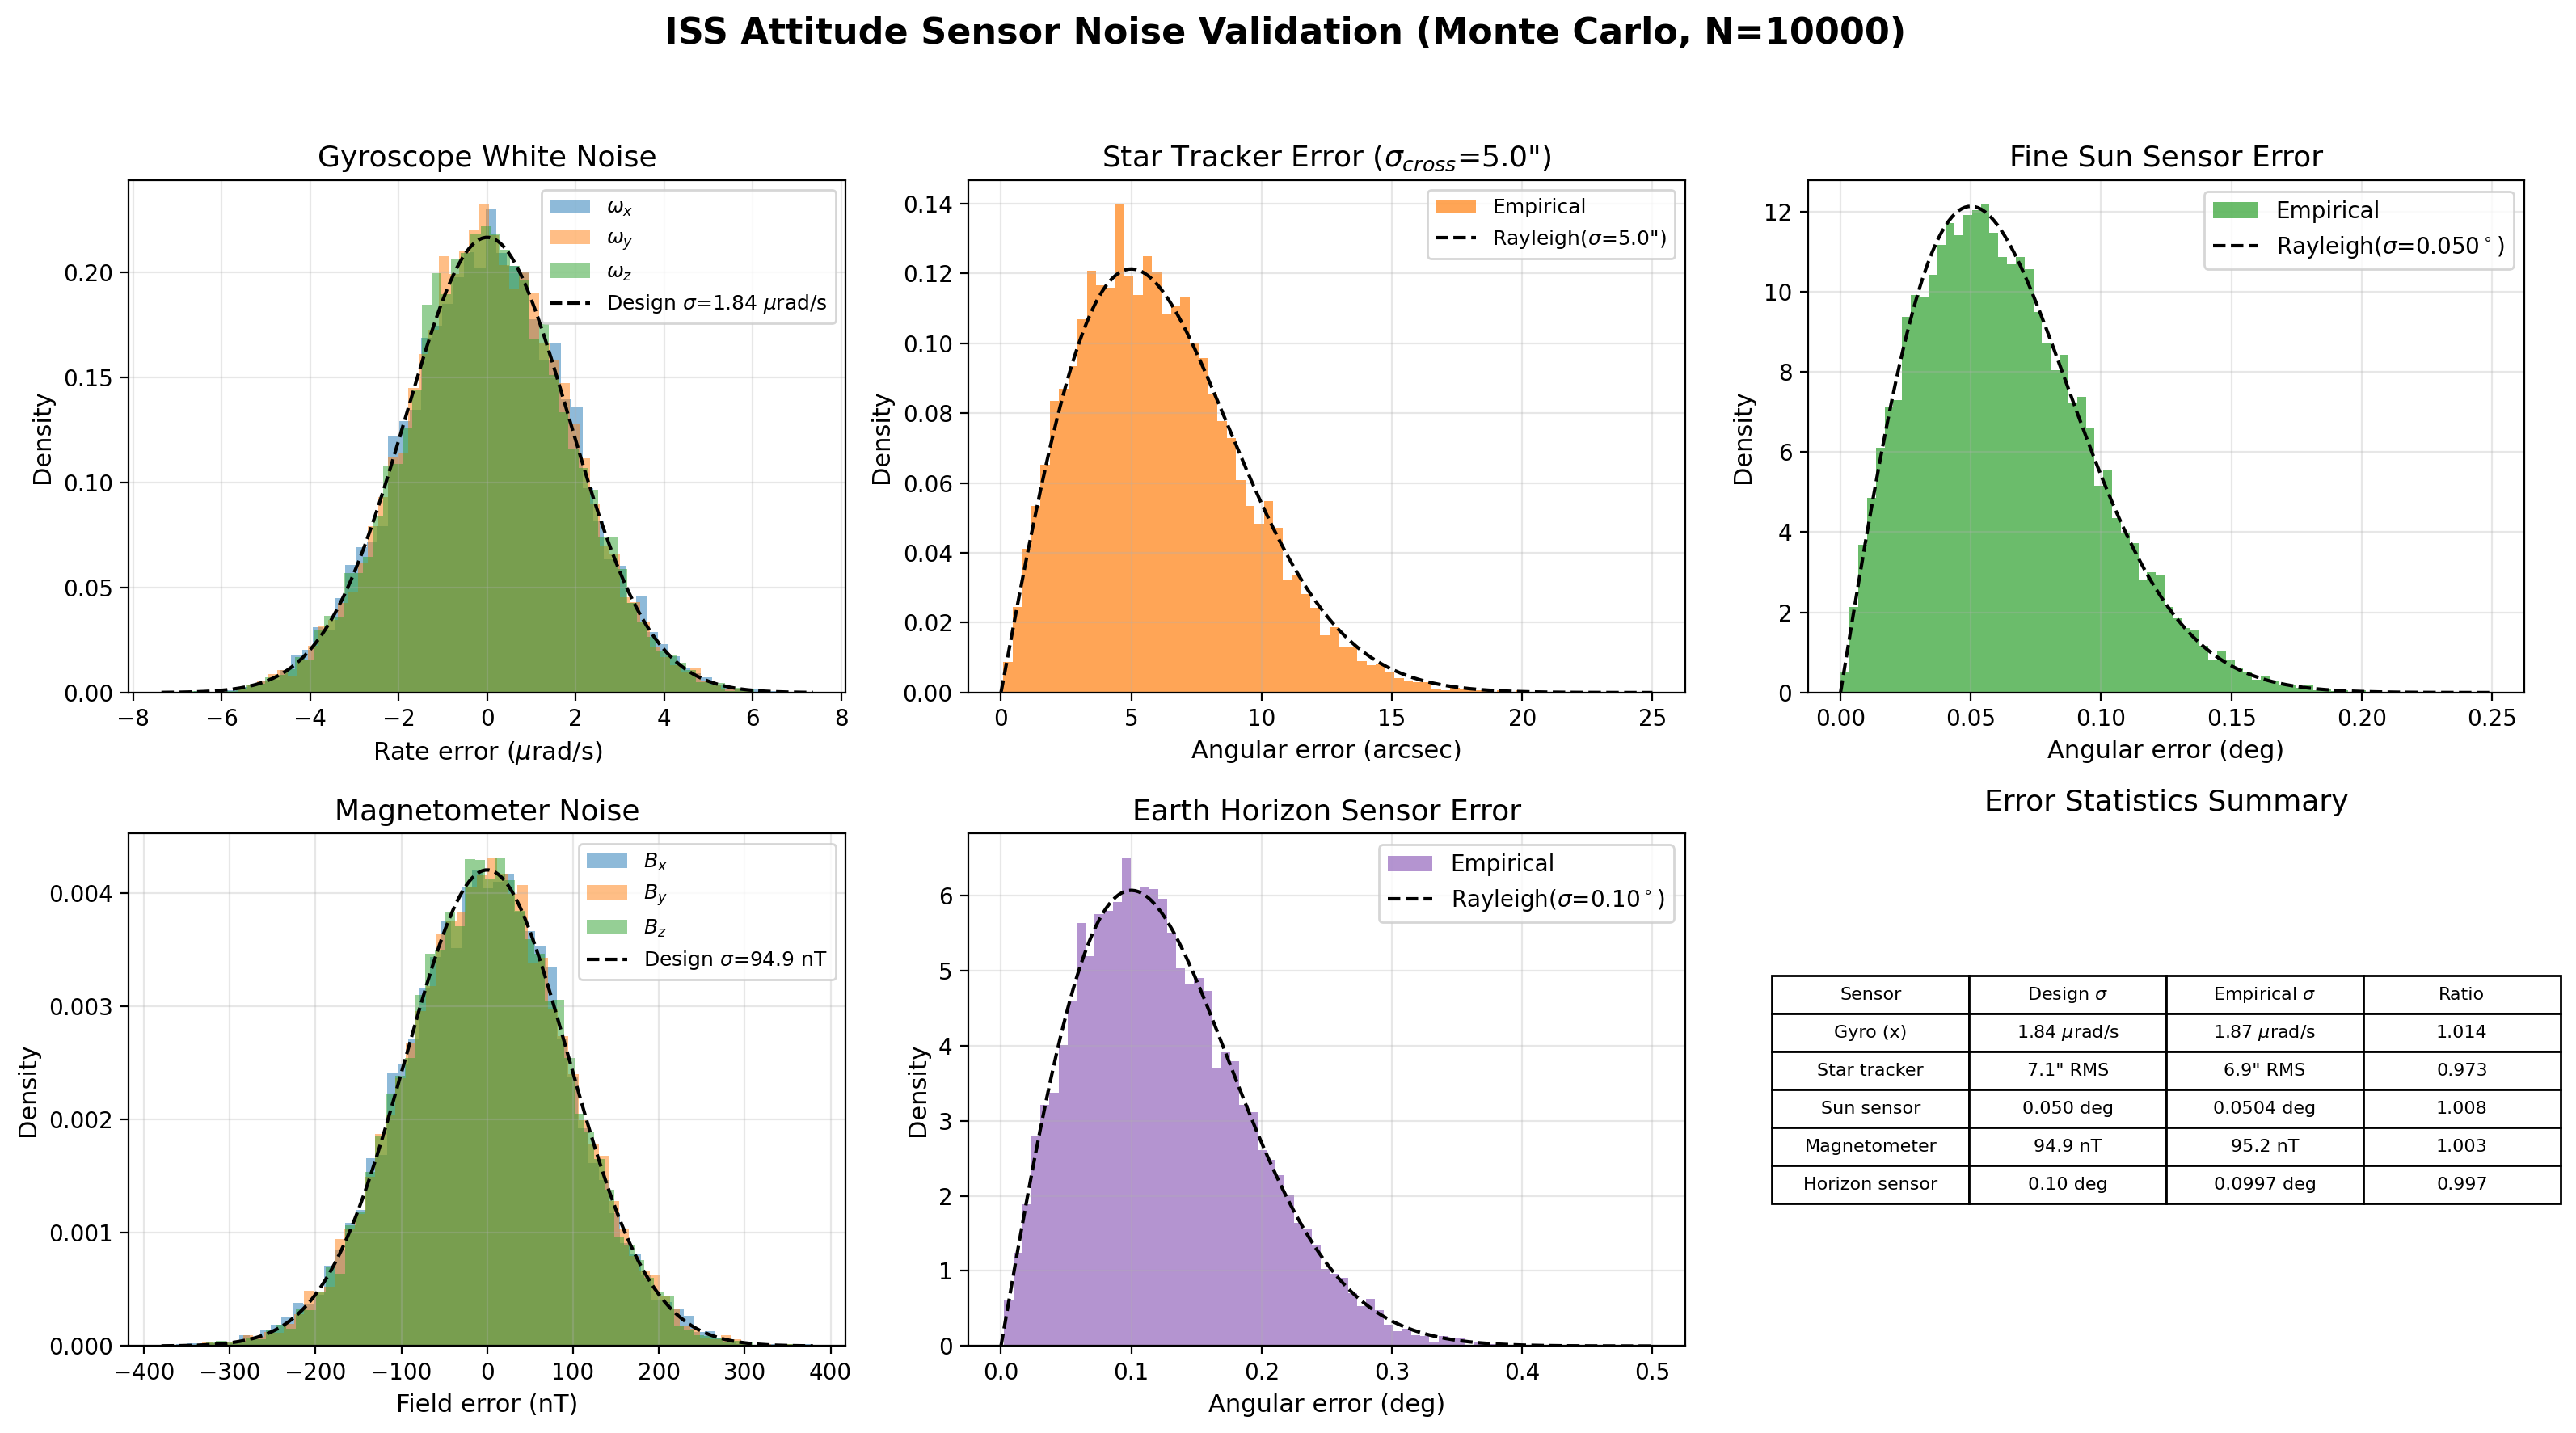
\includegraphics[width=\columnwidth]{attitude_sensors.png}
  \caption{Monte Carlo validation of sensor noise models.  Histograms show
    empirical error distributions; dashed lines show the design distributions.
    All ratios (empirical/design $\sigma$) are within 1--2\% of unity.}
  \label{fig:sensor_validation}
\end{figure}

Fig.~\ref{fig:sensor_validation} confirms all sensor noise models produce
error statistics consistent with the design specifications.  The empirical-to-design
$\sigma$ ratios are all within 2\% of 1.0 across $10{,}000$ trials.

\begin{figure}[t]
  \centering
  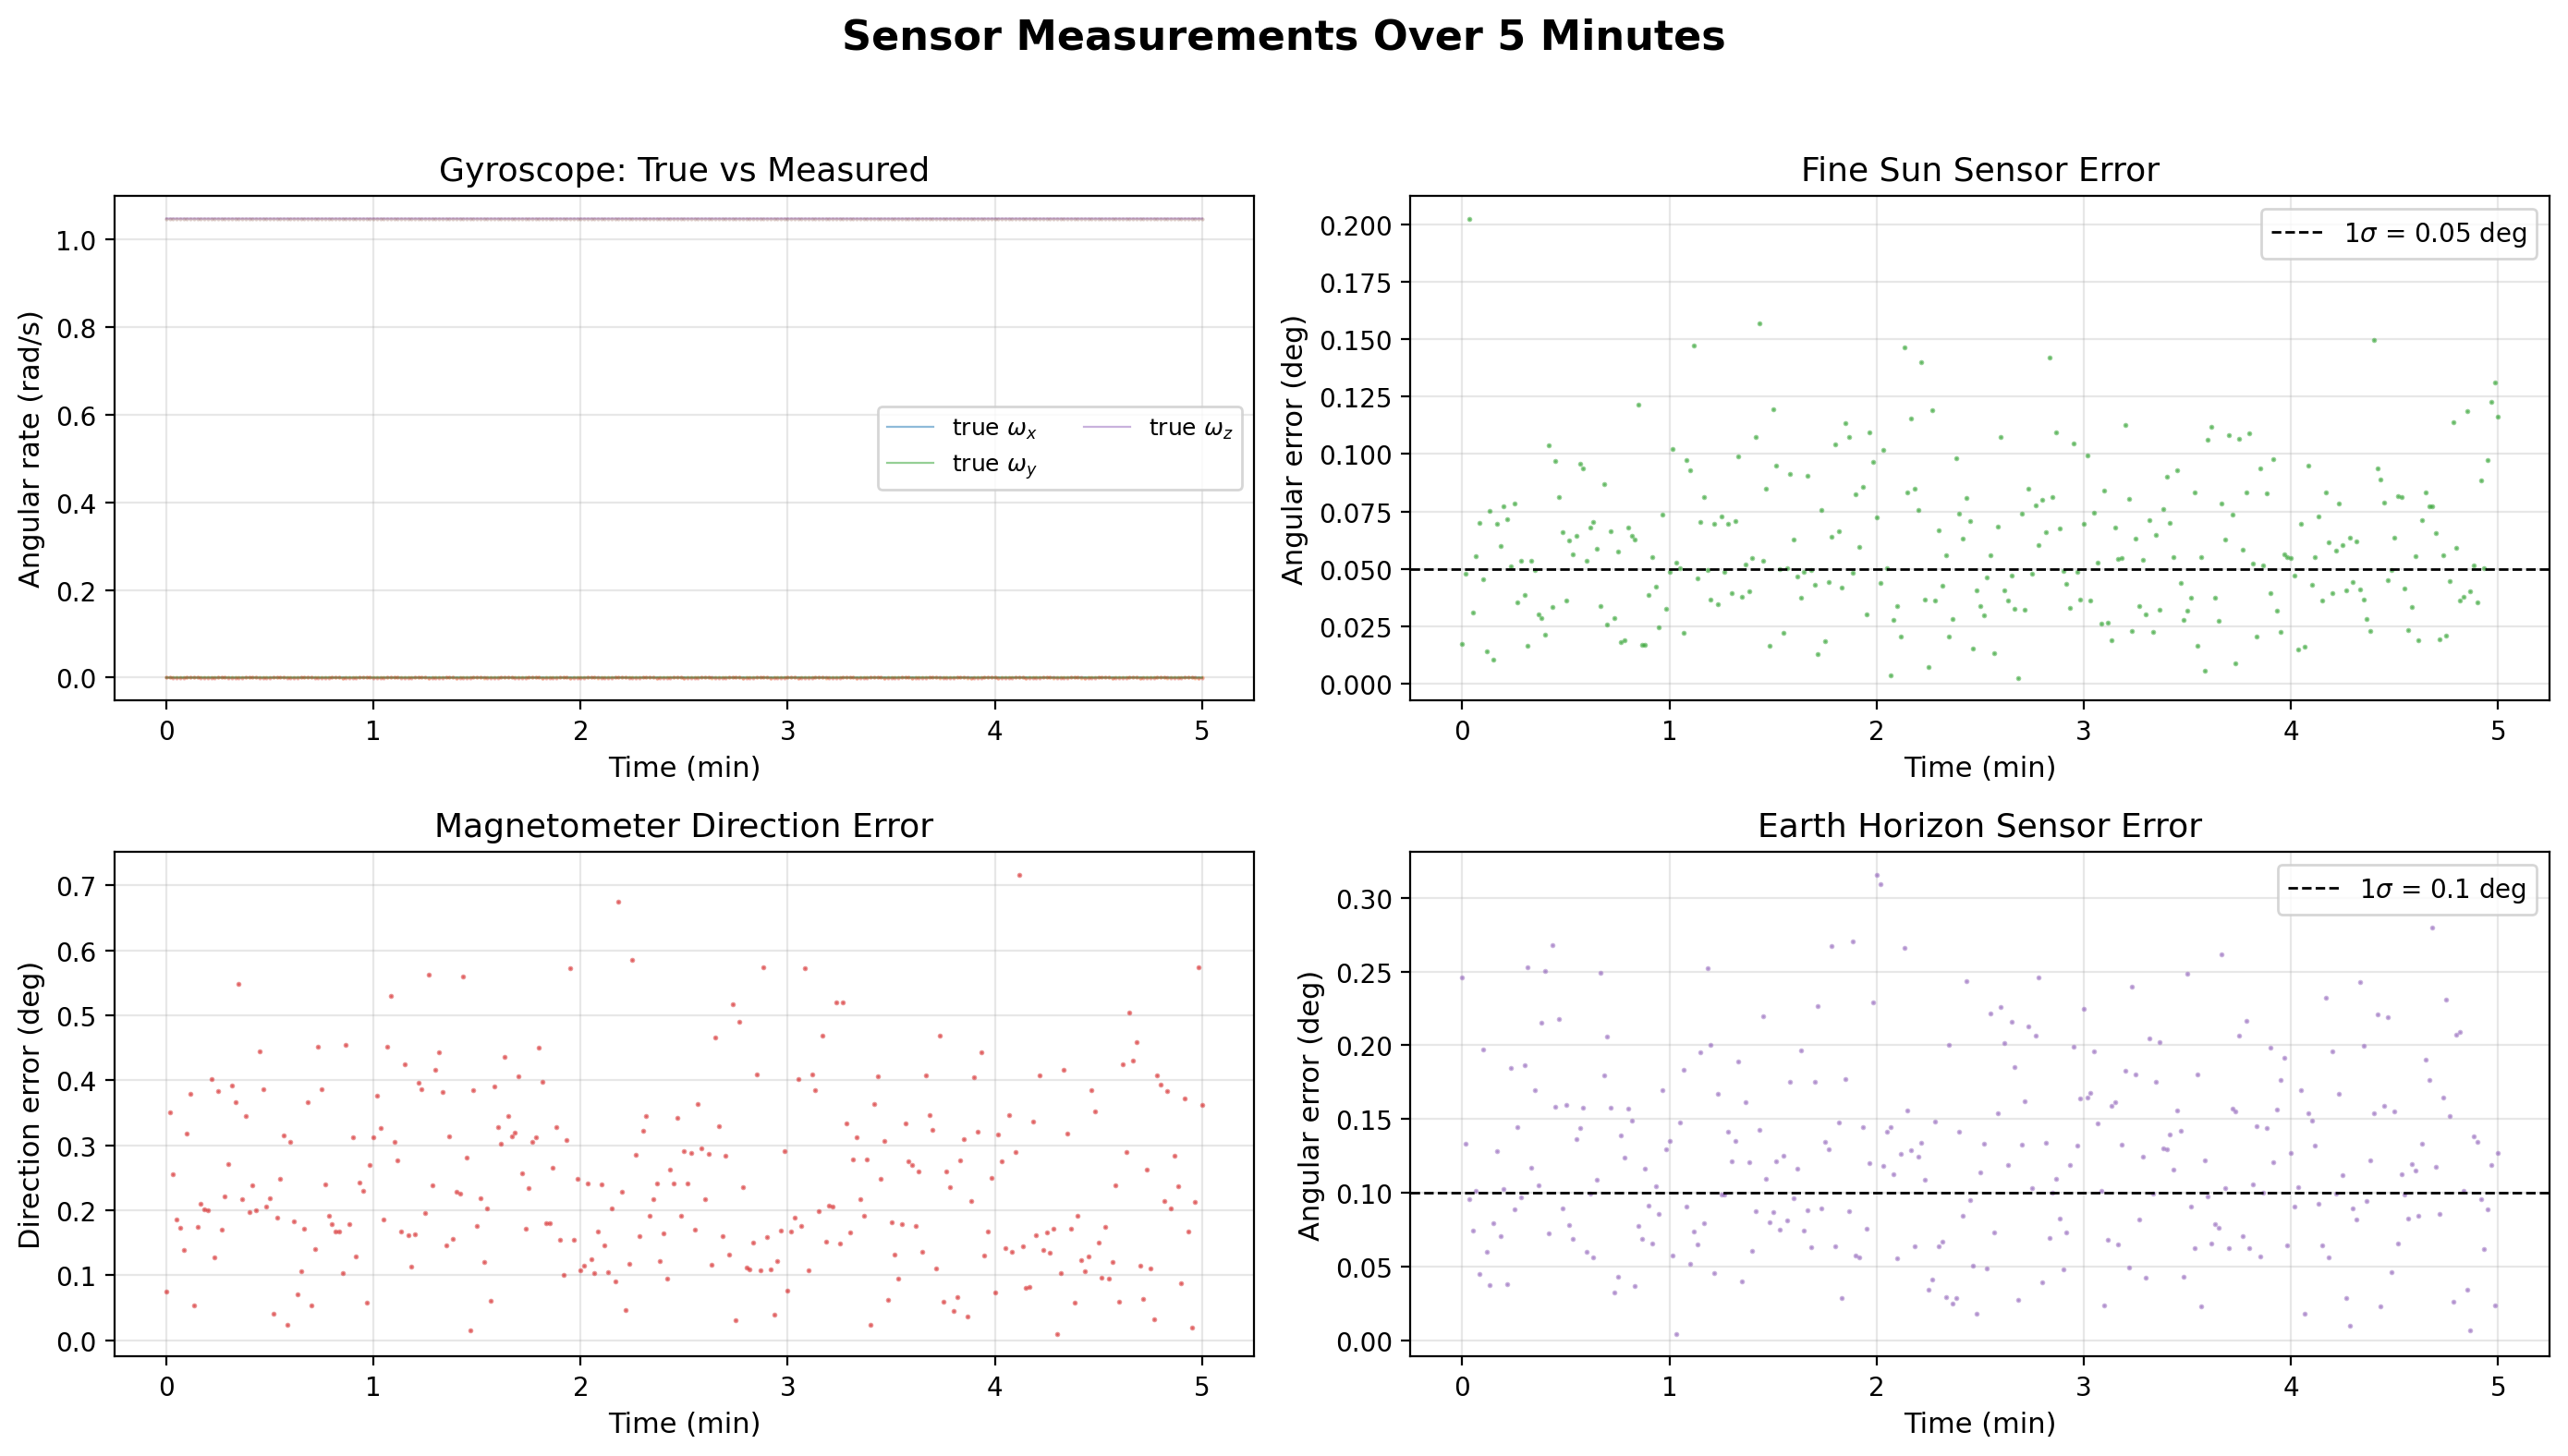
\includegraphics[width=\columnwidth]{attitude_sensors_timeseries.png}
  \caption{Time series of sensor measurements over a 5-minute simulation.
    Gyro measurements track the true angular velocity with sub-$\mu$rad/s noise.
    Direction sensors show errors consistent with their design $\sigma$ values.}
  \label{fig:sensor_timeseries}
\end{figure}

% ------------------------------------------------------------------
\section{Static Attitude Estimation}
\label{sec:wahba}

Static attitude is estimated by solving Wahba's problem~\cite{wahba1965}:
\begin{equation}
  \min_R \sum_i a_i \| \bm{b}_i - R\bm{r}_i \|^2,
  \quad a_i = 1/\sigma_i^2,
\end{equation}
where $\bm{b}_i$ are body-frame observations and $\bm{r}_i$ are reference
(ECI) directions.

\subsection{Algorithms}

\textbf{Davenport's q-method}~\cite{davenport1968}:
The attitude profile matrix $B = \sum a_i \bm{b}_i \bm{r}_i^T$ is converted
to the $4 \times 4$ Davenport matrix $K$.  The optimal quaternion is the
eigenvector of $K$ corresponding to its maximum eigenvalue.
Complexity: $O(1)$ after building $B$.

\textbf{SDP relaxation}~\cite{sdp_wahba}:
Wahba's problem is reformulated as maximizing $\text{tr}(K Q)$ subject to
$Q \succeq 0$, $\text{tr}(Q) = 1$.  This semidefinite relaxation is tight
for Wahba's problem (the optimal $Q$ is always rank-1), so the SDP yields
the exact solution.  Solved using CLARABEL via CVXPY.

\subsection{Monte Carlo Comparison}

Each trial uses five observations: two star directions, one sun direction,
one nadir direction, and one magnetic field direction.  The observation
weights are $1/\sigma_i^2$ based on each sensor's angular noise.

\begin{table}[t]
\centering
\caption{Wahba's Problem: Monte Carlo Results ($N = 5{,}000$)}
\label{tab:wahba}
\begin{tabular}{@{}lcc@{}}
\toprule
\textbf{Metric} & \textbf{q-method} & \textbf{SDP} \\
\midrule
Mean error (arcsec) & 7.04 & 7.04 \\
Median error (arcsec) & 6.55 & 6.55 \\
RMS error (arcsec) & 7.81 & 7.81 \\
Max error (arcsec) & 23.80 & 23.80 \\
Time per solve (ms) & 0.024 & 1.613 \\
Speedup & --- & $67\times$ slower \\
\bottomrule
\end{tabular}
\end{table}

\begin{figure}[t]
  \centering
  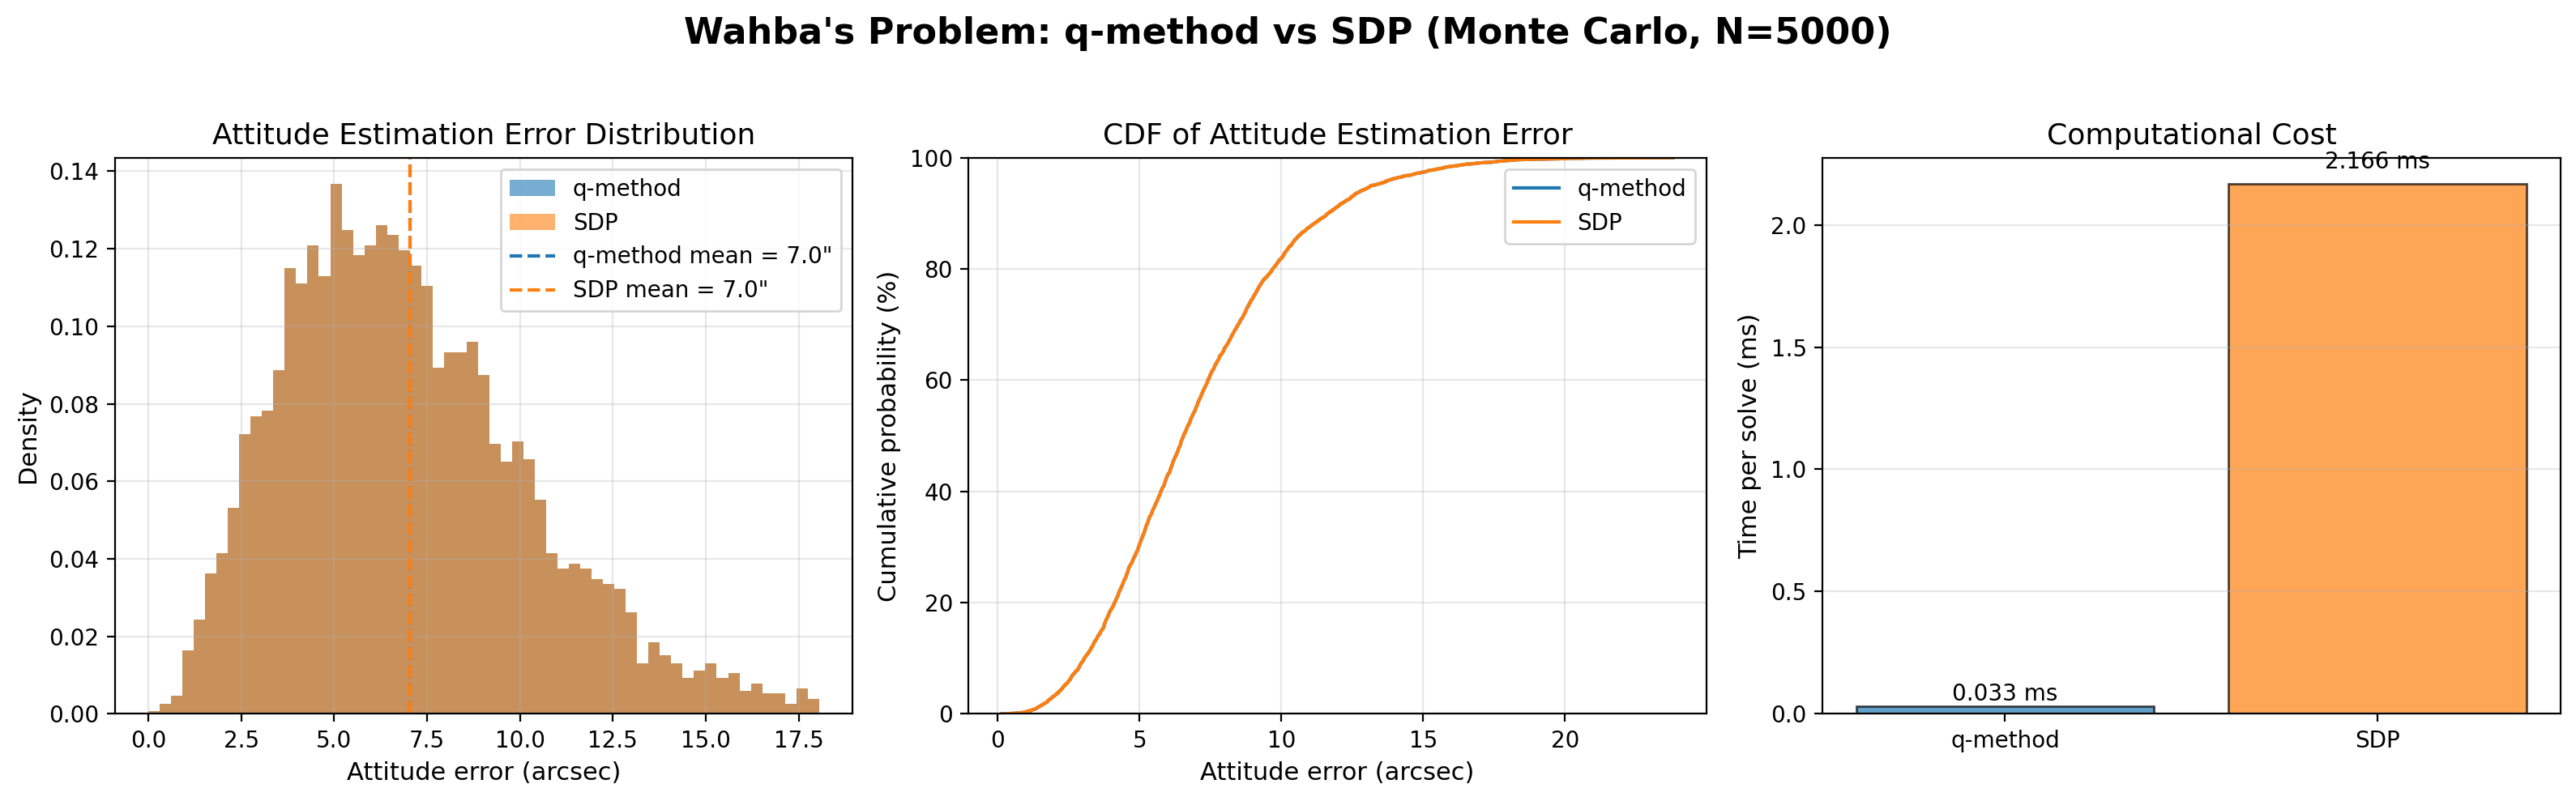
\includegraphics[width=\columnwidth]{attitude_estimation.png}
  \caption{Wahba's problem results.  Left: error histograms (both algorithms
    are identical).  Center: CDF of attitude error.  Right: computational
    cost comparison showing the q-method is $67\times$ faster.}
  \label{fig:wahba}
\end{figure}

Table~\ref{tab:wahba} and Fig.~\ref{fig:wahba} show that both algorithms
produce identical attitude estimates (mean error \SI{7.04}{arcsec}, RMS
\SI{7.81}{arcsec}).  This confirms the SDP relaxation is tight, as expected
for Wahba's problem.  The q-method is $67\times$ faster ($\SI{0.024}{ms}$
vs.\ $\SI{1.613}{ms}$ per solve), making it the preferred choice for
real-time applications.

% ------------------------------------------------------------------
\section{Changelog}

\begin{table}[h]
\centering
\begin{tabular}{@{}ll@{}}
\toprule
\textbf{Date} & \textbf{Description} \\
\midrule
2026-03-12 & HW2: Safe mode, dynamics, sensors, estimation \\
2026-02-26 & HW1: Mission description, model, dynamics, Euler \\
\bottomrule
\end{tabular}
\end{table}

\begin{thebibliography}{9}
\bibitem{nasa_iss}
NASA, ``International Space Station: Facts and Figures,''
\url{https://www.nasa.gov/feature/facts-and-figures}, 2024.

\bibitem{wahba1965}
G.~Wahba, ``A least squares estimate of satellite attitude,''
\textit{SIAM Review}, vol.~7, no.~3, p.~409, 1965.

\bibitem{davenport1968}
P.~B.~Davenport, ``A vector approach to the algebra of rotations
with applications,'' NASA TN D-4696, 1968.

\bibitem{sdp_wahba}
F.~L.~Markley and J.~L.~Crassidis,
\textit{Fundamentals of Spacecraft Attitude Determination and Control}.
New York: Springer, 2014, ch.~5.

\bibitem{honeywell_gg1320}
Honeywell, ``GG1320AN Digital Ring Laser Gyroscope,'' datasheet, 2020.

\bibitem{sodern_sed36}
Sodern, ``SED36 Star Tracker,'' product specification, 2019.

\bibitem{adcole}
Adcole Corporation, ``Two-Axis Digital Sun Sensor,'' datasheet.

\bibitem{honeywell_hmc2003}
Honeywell, ``HMC2003 Three-Axis Magnetic Sensor Hybrid,'' datasheet, 2018.

\bibitem{smad}
J.~R.~Wertz and W.~J.~Larson,
\textit{Space Mission Analysis and Design}, 3rd ed.
Microcosm Press, 1999.
\end{thebibliography}

\end{document}
